%\documentclass{article}
%\usepackage{graphicx,subfigure}
%\begin{document}

\begin{figure}[h]
  \centering
   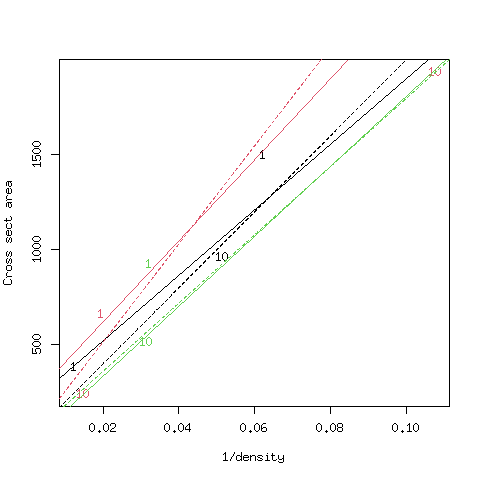
\includegraphics[width=0.9\textwidth]{DC1955/expt1reg.png}
  \caption{Plot of breed means for reciprocal of follicle density and fibre cross sectional area from Daly and Carter(1955)~\cite{daly:55} experiment 1. The black lines are linear regressions fitted to all data, full line with an intercept, dashed line without an intercept. The red lines are linear regressions fitted to breed means for period 1 . The green lines are linear regressions fitted to breed means for period 10 .}
  \label{fig:dcexpt1reg}
\end{figure}

%\end{document}

